\documentclass{article}
\usepackage[utf8]{inputenc}
\usepackage[margin=1.0in]{geometry}
\usepackage[bottom]{footmisc}
\usepackage{graphicx}
\usepackage{hyperref}
\usepackage{mathtools}
\usepackage{amsmath}
\usepackage{tcolorbox}
\usepackage{subcaption}
\usepackage{float}
\usepackage{multirow}
\usepackage{titlesec}
\setcounter{secnumdepth}{5}
\usepackage[toc,page]{appendix}

\title{Results}
\date{June 2020}

\begin{document}

\maketitle
% Lotka-Volterra goes here

Having established theoretical understandings of Monte Carlo and Kalman Filter methods, as well as seen their application to two biological systems, it is now necessary to compare the techniques in various situations. Additionally, we now include Particle Swarm Optimization (PSO) as a third technique for parametrization that we will consider. We will perform our comparisons first on the Lotka-Volterra system and then on the T1D model.

\section{Lotka-Volterra}


\section{Type 1 Diabetes}

\subsection{Approach To Comparisons}

In the context of the T1D model, we will compare the MCMC, UKF, and PSO approaches on both a population and individual level. Recall that for the T1D Model we use data from 11 different mice, 9 of which we classified as acute and 2 of which we classified as progressive as in section \ref{section:Individual_data}. For our population comparison, we will show fits done on an average of all the data from the acute mice, and for the individual level comparison, we will compare fits done on Mouse 6. We choose to compare the algorithms' performances in two different contexts in order to gain an understanding of the algorithms' performance in various situations. We hope that this will allow us to determine when a certain algorithm would be preferable over its counterparts.


\subsection{Individual Level Comparison}
To perform an individual-level comparison, we utilize mouse 6 as an example. As explained when utilized by the UKF algorithms, mouse 6 has been determined in an ad hoc fashion to be a good representation of the population as a whole as it provides us with 10 raw data points, significantly more than the average of ***. To get the Kalman Filter fits we use the standard approach used thus far of performing five iterations and choosing the best based on MSE value. Next, for MCMC we now run the algorithm using \emph{just} mouse 6 data, instead of the averaged Li data as was done previously. Finally, for PSO we run the algorithm, just as with MCMC, on the mouse 6 data only. To assess quality of fit, we use the same visual and numerical criteria of plotting fits and considering RMSE values as before. 
\begin{figure}[H]
    \centering
    \includegraphics[width=15cm]{Comparison_Figures/Mouse6_ComparisonFigure.jpg}
    \caption{Plot of raw mouse 6 data overlayed with MCMC, UKF, and PSO fits. It is evident that there is range of success on the individual mouse, with PSO appearing to perform best.}
    \label{fig:Results_Mouse6_Comparison}
\end{figure}
Visually, as seen in Figure \ref{fig:Results_Mouse6_Comparison}, it is reassuring to see that we achieve similar results across the 4 algorithms. We mean this in the sense that every algorithm follows a similar shape and appears to predict similar onset times. However, we do see a difference in starting behavior where the PSO, MCMC, and Dual UKF all start with glucose around 100 $\frac{mg}{dL}$ then show a decrease before the slow steady increase, while the Joint UKF immediately begins its increase. Interestingly, it appears that after increasing to glucose of around 175 $\frac{mg}{dL}$, the prediction levels off or possibly even decreases very slightly until it reaches its pivot point. Overall, we see visually that the PSO algorithm appears to fit the raw data the best. However, there is an odd angle occurring at the pivot point in the PSO prediction. This should be a smooth curve as the others illustrate and it is not quite clear to us what is causing this angle. Despite this odd shape, we again use the root mean squared error of each algorithm to score performance.
\begin{table}[H]
  \begin{center}
    \label{tab:table1}
    \begin{tabular}{c|c} % <-- Alignments: 1st column left, 2nd middle and 3rd right, with vertical lines in between
      \textbf{Algorithm} & \textbf{RMSE} \\
      \hline
      \textbf{MCMC} & 66.8\\
      \textbf{PSO} & 28.2\\
      \textbf{Dual UKF} & 50.2\\
      \textbf{Joint UKF} & 67.1
    \end{tabular}
    \caption{Root Mean Squared Error (RMSE) of ODE simulations using parameter estimates to fit to Li mouse 6 data. The quantification of the error confirms our visual hypothesis that PSO performs the best fit on this data set.}
    \label{table:Results_Mouse6_RMSE}
  \end{center}
\end{table}
Table \ref{table:Results_Mouse6_RMSE} confirms that the PSO algorithm is indeed fitting the raw data the best. We note that the Dual UKF is outperforming the MCMC algorithm and while the MCMC scores better than the Joint UKF method, the two scores are very similar. This also lends support to our assertion that the Dual UKF normally outperforms the Joint UKF. 


\subsection{Population Level Comparisons}

\subsubsection{Comparison of Averaging Techniques}
The averaged version of the Li et al dataset was produced as in section \ref{section:population_level_data} in order to understand the predicted behavior of a general mouse in the cohort. In dealing with the average data, we consider two approaches to fitting this dataset:
\begin{enumerate}
    \item Average Then Fit: Run algorithm on the already averaged dataset.
    \item Fit Then Average: Run algorithm on each mouse individually and then average the parameter values
\end{enumerate}
In the first scenario, we treat the averaged data as a new dataset, as was done in the for the traditional MCMC fits. However, in our second option, we fit to every mouse individually, as was performed in the UKF section \ref{section:UKF_T1D_Implementation} and then treat averages of those parameters as the new final parameters. For example, a parameter value for $G_I$ is found for every mouse, and then the mean of these values is used to understand the population. Thus, in this case the algorithms never work with the averaged dataset directly. We chose to test both approaches since the UKF has not historically been used with averaged data. As a result, we are not initially sure which approach would work best and thus attempt both to allow us to know in the future how best to deal with averaged data. First, let's consider scenario one on the MCMC and PSO algorithms. This represents the standard way one would use averaged data as has been done throughout the paper thus far.


%{In order to compare the algorithms at a population level, we use average acute mice data as prepared in section X. Then, we produce the following four fits to this data. First, we use the mean parameters from the MCMC posterior distributions achieved from running the algorithm on this data set. Next, the second and third fits come from averaging the final parameter values achieved on the set of acute mice from the Joint and Dual UKF algorithms. For example, a final value of $\eta$ was produced by running the algorithms on each mouse. Now, we average all of those $\eta$ values to produce a population-level parameter. Our fourth fit is from running the PSO on the population level data. In order to assess the goodness of fit, we plot the fits on top of one another along with the raw data for a visual check and also compare the MSE values. %}


\subsubsection{Average First with MCMC and PSO}
\begin{figure}[H]
    \centering
    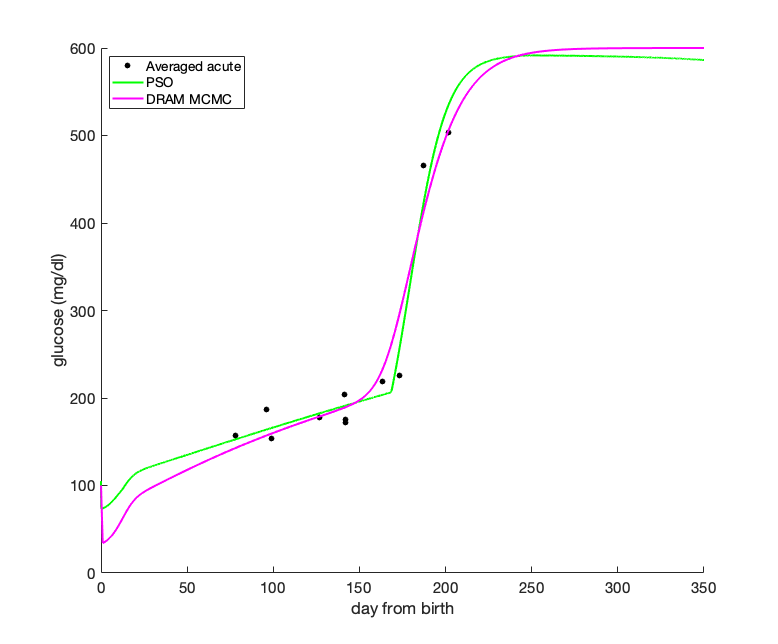
\includegraphics[width=15cm]{Comparison_Figures/averagethenfit_pso_dram_comp.png}
    \caption{Plot of averaged acute Li data overlayed with PSO and DRAM MCMC fits. This figure illustrates the results of averaging data then fitting.}
    \label{fig:Results_Averaged_PSOMCMC_Fits}
\end{figure}
From Figure \ref{fig:Results_Averaged_PSOMCMC_Fits}, both algorithms are doing a fair job of capturing the raw averaged data. We are unsurprised at the goodness of fit from the DRAM MCMC algorithm as many studies utilize MCMC methods to parameterize on large often averaged data sets. The PSO fit provides us with a loose validation that averaging data before parameterizing does indeed produce satisfactory results. We look to the root mean squared error scores to provide us with more comparative information between algorithms.
\begin{table}[H]
  \begin{center}
    \label{tab:table1}
    \begin{tabular}{c|c} % <-- Alignments: 1st column left, 2nd middle and 3rd right, with vertical lines in between
      \textbf{Algorithm} & \textbf{RMSE} \\
      \hline
      \textbf{PSO} & 35.46\\
      \textbf{DRAM MCMC} & 30.71\\
    \end{tabular}
    \caption{Root Mean Squared Error (RMSE) of ODE simulations using PSO and DRAM MCMC. Each algorithm was run on pre-averaged acute data.}
    \label{table:Results_Averaged_PSOMCMC_RMSE}
  \end{center}
\end{table}
While the root MSE tells us that the DRAM MCMC algorithm performed slightly better than the PSO method, the scores are not significantly different. While not a perfect fit of the data, we are satisfied that both algorithms have performed well. These results help us to confirm that averaging data before parameterization is a good method for producing biologically feasible results.
\subsection{Average First verus Fit First}
UKF algorithms have traditionally been used on individual-level data. Thus, there are no established techniques from literature for how to utilize averaged data. One obvious approach is option 1. However, due to our hypothesis that UKF's are better suited for option 2, we thus attempt to perform the fit this way as well. Once again, we use the PSO as a tool for comparison.

\begin{figure}[H]
    \centering
    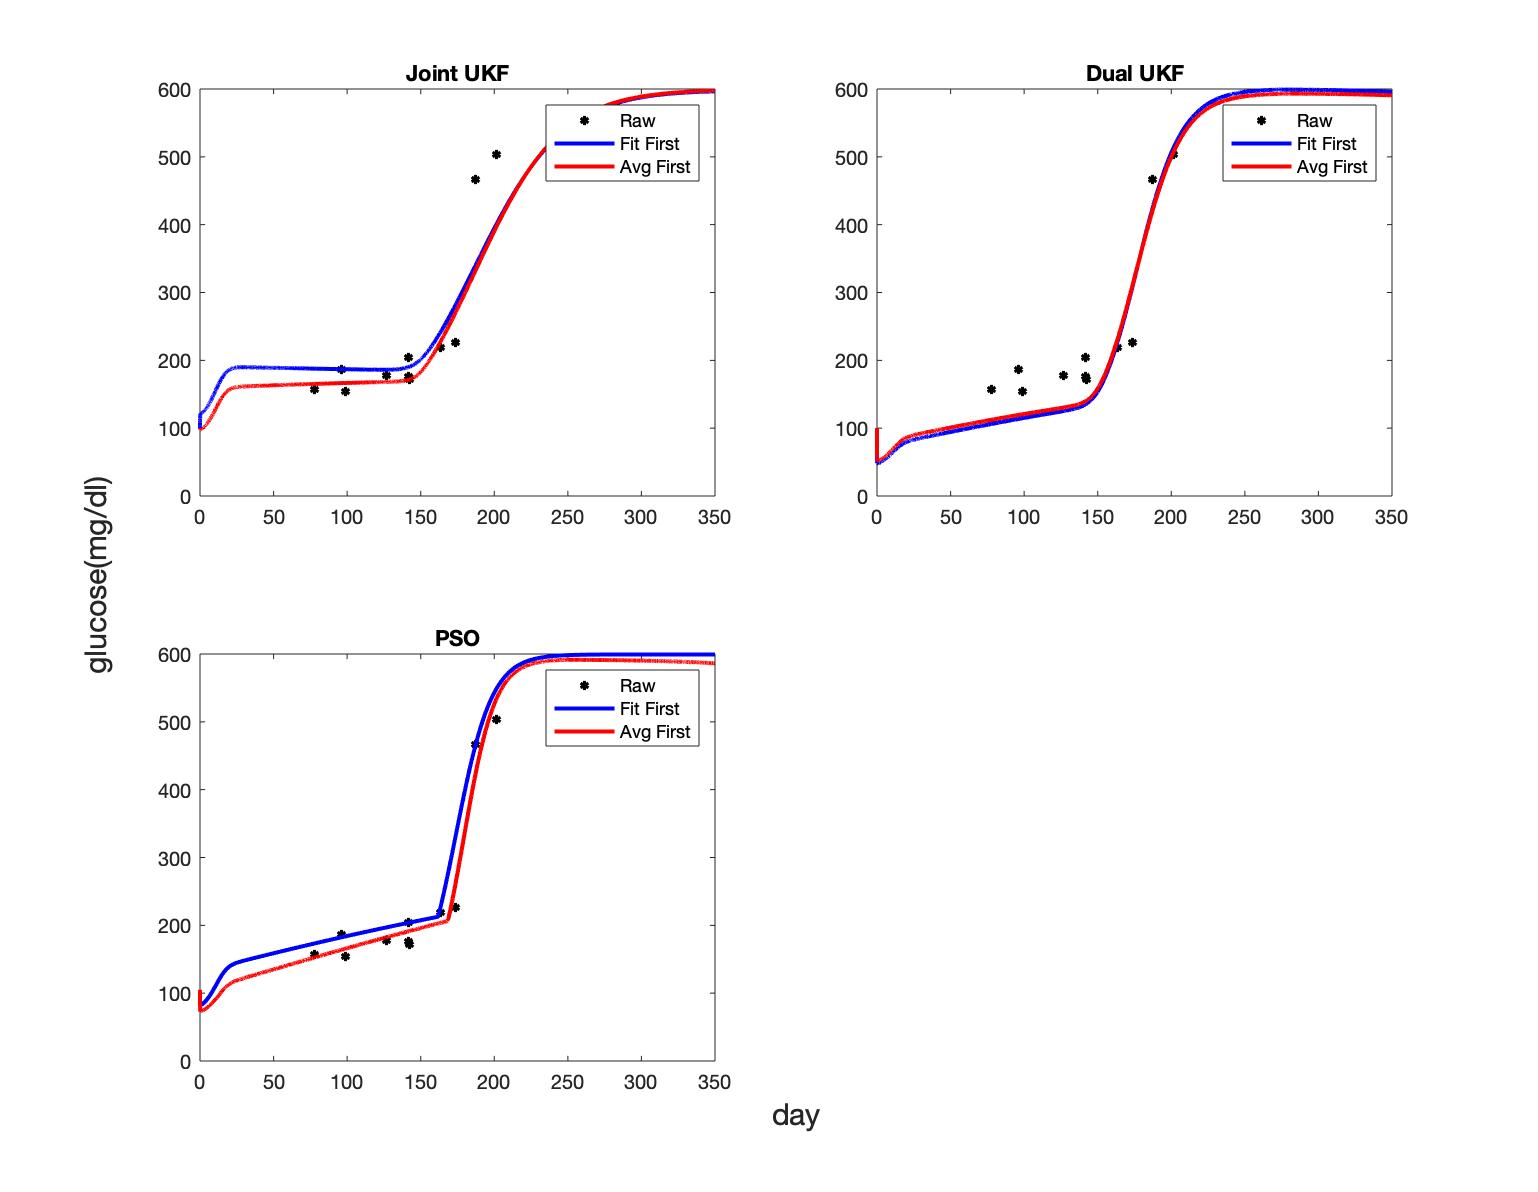
\includegraphics[width=15cm]{Comparison_Figures/FitFirst_vs_AvgFirst_PSOUKF.jpg}
    \caption{Plots of using Joint and Dual UKFs, as well as PSO, to fit to averaged Li data by both running the algorithms directly on this dataset as well as by averaging parameters from individual fits instead of training on the actual averaged dataset. It is evident that averaging first produces slightly better results for PSO and the Joint UKF. For the Dual UKF, the fits are so similar it is hard to see which is better.}
    \label{fig:Results_FitFirstAvgFirst_Comparison}
\end{figure}
Looking at the PSO fits first, the difference in technique does not appear to alter results significantly. A slight advantage is seen in averaging first, however by no means a drastic one. This is corroborated by both the Joint and Dual UKF fits. Thus, it appears that if one's intention is to work with averaged data, training directly on the averaged data may provide a slight advantage, but there is overall little difference. More importantly, as compared to the UKF fits in section \ref{section:T1D_DualUKF_Results}, which were performed on data form a single mouse, the performance here appears worse. This confirms our hypothesis that UKF's perform better on individual-level data, and we will soon see a potentially more effective way to incorporate UKF methods as part of a fit to averaged data in section \ref{section:Combining_UKF_MCMC}.

\subsection{Fit First Comparison Results}
To further understand the quality of fit when using parameters averaged from individual mouse fits, we can plot the result of this technique using the Joint UKF, Dual UKF, and PSO all together, as well as now consider their RMSE values in Figure \ref{fig:Results_FitFirst_Comparison} and Table \ref{table:Results_FitFirst_RMSE}.
\begin{figure}[H]
    \centering
    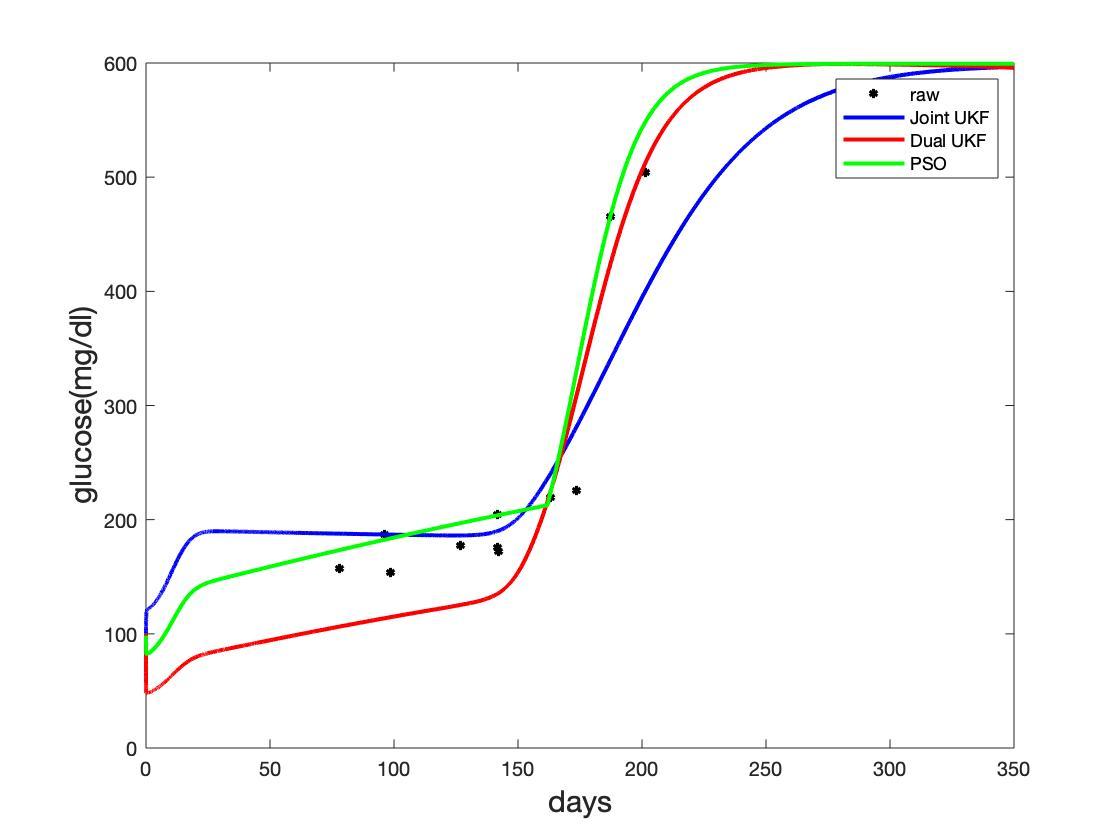
\includegraphics[width=15cm]{Comparison_Figures/Fit_Then_Average_Figure.jpg}
    \caption{Plot of using Joint UKF, Dual UKF, and PSO to fit to averaged Li data by averaging parameters from individual fits instead of training on the actual averaged dataset. It is evident that the PSO once again performs best, whereas the Joint UKF captures the early behavior accurately and then struggles and the Dual UKF struggles early but captures the end behavior.}
    \label{fig:Results_FitFirst_Comparison}
\end{figure} 

\begin{table}[H]
  \begin{center}
    \label{tab:table1}
    \begin{tabular}{c|c} % <-- Alignments: 1st column left, 2nd middle and 3rd right, with vertical lines in between
      \textbf{Algorithm} & \textbf{RMSE} \\
      \hline
      \textbf{PSO} & 35.46\\
      \textbf{Joint UKF} & 52.07\\
      \textbf{Dual UKF} & 51.06
    \end{tabular}
    \caption{Root Mean Squared Error (RMSE) of ODE simulations using PSO and DRAM MCMC. Each algorithm was run on pre-averaged acute data.}
    \label{table:Results_FitFirst_RMSE}
  \end{center}
\end{table}

Both visually and numerically, it is evident that PSO performs best on this dataset. Overall, this analysis suggests that using UKF's directly on averaged data, whether by fitting first or averaging first, is most likely not an optimal approach. 




\end{document}



%THIS MIGHT GO SOMEWHERE
%{\par It is interesting to note that the PSO algorithm performs the best on both data sets. The MCMC algorithm seems to do better on the averaged data while the UKF methods overall tended to perform better on the single mouse 6 data. The fact that UKF methods are more successful on the mouse 6 data may be attributed to the fact that the UKF is tuned to the specific system it is estimating. Because of this, the UKF is searching for the specific parameters of the system, as opposed to the MCMC which is searching for a distribution of parameters. Since the parameters are biological, we assume that there might be slight differences between the actual parameters for different mice, and indeed we found earlier that when running the UKF on different mice, we get different results. However, when working with average data, there is not necessarily going to be one set of parameters that describe the system perfectly, which hurts the UKF since it is trying to adapt itself to the system. %}